% ----------------------------------------------------------
\section{Monitoramento de referência da qualidade do ar}
% ----------------------------------------------------------

As redes de referência são compostas por estações de monitoramento, certificadas por órgãos competentes, as quais registram ininterruptamente, e em tempo real, as concentrações dos poluentes na atmosfera \cite{CETESB2020RedesAr}. As estações podem ser fixas ou móveis e a qualidade das suas leituras é garantida mediante procedimentos padrões de calibração dos instrumentos, de coleta de dados e de pós-processamento. As informações coletadas pelas estações da rede são enviadas a um computador central, na forma de médias horárias, por meio de sistemas de telemetria. Ali os dados são processadas com base nos padrões legais estabelecidos e podem ser disponibilizados na forma de boletins diários ou relatórios anuais, como um resumo das condições da poluição atmosférica dentro de determinada área \cite{CETESB2020RedesAr}. Os métodos de medição de referência utilizados para cada poluente nas estações são documentados no Guia Técnico para o Monitoramento e Avaliação da Qualidade do Ar \cite{Franca2019GUIAAR}, e resumem-se na Tabela \ref{tab:monit-methods}.

\begin{table}[h]
    \caption{Metodologias de monitoramento de referência}
    \centering
    \begin{tabularx}{0.95\textwidth}[h]{
         >{\raggedright\arraybackslash}X
         >{\raggedright\arraybackslash}X }
        \textbf{Poluentes} & \textbf{Métodos de Medição} \\
        \hline
        Partículas totais em suspensão & Amostrador de Grande Volume (AGV) \\
        \hline
        Dióxido de enxofre & Fluorescência na região ultravioleta \\
        \hline
        Dióxido de nitrogênio & Quimiluminescência em fase gasosa \\
        \hline
        Monóxido de carbono & Fotometria infravermelha não dispersiva \\
        \hline
        Ozônio & Quimiluminescência \\
        \hline
        Fumaça & Refletância da luz \\
        \hline
    \end{tabularx}
    \label{tab:monit-methods}
    \fonte{\cite{Franca2019GUIAAR}}
\end{table}

As redes de monitoramento de referência caracterizam-se por uma elevada precisão e confiabilidade. Contudo, fatores como preço, consumo energético, complexidade de operação e de instalação dificultando seu uso de forma mais extensa. A literatura reporta preços dessas tecnologias em torno de \$ 15.000 – \$ 100.000 \cite{Concas2021LOW-COSTPREPRINT} e consumo de potência aproximadamente entre 0.2 e 1 kW \cite{Piedrahita2014TheMonitoring}, sem contar os custos advindos dos procedimentos de instalação, operação e manutenção \cite{Kumar2015,Ferreira2022}. Sendo assim, a onerosidade da solução como um todo limita o número de estações financeiramente viáveis e reduz a resolução e distribuição espacial das medições, inclusive em países e regiões com elevados índices de desenvolvimento econômico como os Estados Unidos e a Europa \cite{Kumar2015,Jiao2016CommunityStates}.

No Brasil o monitoramento de referência é ainda bastante limitado. Algumas iniciativas governamentais e de órgãos de pesquisa, a nível nacional e estadual, têm sido implementadas para facilitar o acesso a dados sobre a qualidade do ar como, por exemplo: \cite{CETESB2020RedesAr}, \cite{IEMA2020QualidadeAr} e \cite{IEMA/ES2020IEMAAr}. No entanto, ainda assim, as redes de monitoramento que têm sido instaladas cobrem escassos pontos das cidades brasileiras e seu desempenho a longo prazo muitas vezes se vê comprometido por falta de manutenção e de pessoal qualificado \cite{Oyama2017AIRBRAZIL}. Estudos realizados entre os anos 2021 e 2022 sobre o estado do monitoramento da qualidade do ar no Brasil apontam que, das 27 unidades federativas, menos da metade (entre 11 - 12) monitoram a qualidade do ar e atendem a regulamentação vigente \cite{Vormittag2021AnaliseBrasil,Ferreira2022}. A Tabela \ref{tab:monit-stations-br}  resume as unidades federativas reportadas em cada trabalho que possuem rede de monitoramento de referência ativas e gerenciadas por algum órgão público ou entidades privadas. Existem algumas inconsistências nos dados mostrados em cada trabalho, já que o número de estações muda de forma abrupta em alguns estados, mas é possível extrair uma visão geral da abrangência das redes de monitoramento no país. As Figuras \ref{fig:monit-stations-br-2021} e \ref{fig:monit-stations-br-2022} mostram mapas com o total de estações em cada região do Brasil conforme foi reportado pelos dois trabalhos mencionados. Observa-se nos mapas que as regiões sul e sudeste concentram quase a totalidade das estações \cite{Vormittag2021AnaliseBrasil,Ferreira2022} e que na região norte, onde se verificam emissões de poluentes em larga escala provindos de incêndios florestais, não há qualquer monitoramento \cite{Ferreira2022}. Vale ressaltar também que, embora não incluído nos dados levantados pelos dois trabalhos anteriores, o estado de Santa Catarina conta na atualidade com 3 estações de monitoramento de referência operadas pela Diamante Geração de Energia Ltda. localizadas nos municípios de Tubarão e Capivari de Baixo. 

\begin{table}[t]
    \caption{Total de estações de monitoramento no Brasil}
    \centering
    \begin{tabularx}{0.95\textwidth}[h]{
         >{\raggedright\hsize=.05\hsize\arraybackslash}X
         >{\raggedright\hsize=.30\hsize\arraybackslash}X 
         >{\raggedright\hsize=.30\hsize\arraybackslash}X
         >{\raggedright\hsize=.30\hsize\arraybackslash}X }
        \textbf{UF} & \textbf{Total de estações privadas}\footnotemark[1] & \textbf{Total de estações públicas (2021)}\footnotemark[1] & \textbf{Total de estações públicas (2022)}\footnotemark[2] \\ [0.5ex] 
        \hline
        AC & 2 & 29 & - \\ [0.5ex]
        \hline
        BA & - & - & 10 \\ [0.5ex]
        \hline
        CE & - & - & 1 \\ [0.5ex]
        \hline
        DF & - & 4 & 5 \\ [0.5ex]
        \hline
        ES & 6 & 9 & 17 \\ [0.5ex]
        \hline
        GO & - & 2 & 2 \\ [0.5ex]
        \hline
        MG & 32 & - & 53 \\ [0.5ex]
        \hline
        MS & 3 & - & 3 \\ [0.5ex]
        \hline
        PE & 3 & 1 & 4 \\ [0.5ex]
        \hline
        PR & - & 16 & 15 \\ [0.5ex]
        \hline
        RJ & 96 & 65 & 91 \\ [0.5ex]
        \hline
        RS & 11 & 2 & 6 \\ [0.5ex]
        \hline
        SP & - & 90 & 79 \\ [0.5ex]
        \hline
    \end{tabularx}
    \label{tab:monit-stations-br}
    \fonte{\cite{Vormittag2021AnaliseBrasil,Ferreira2022}}
\end{table}
\footnotetext[1]{Dados levantados por Vormittag e colaboradores \cite{Vormittag2021AnaliseBrasil}}
\footnotetext[2]{Dados levantados por Ferreira e colaboradores \cite{Ferreira2022}}

\begin{figure}[h]
    \centering
    \caption{Estado do monitoramento de referencia da qualidade do ar no Brasil}
    \begin{subfigure}{0.45\textwidth}
        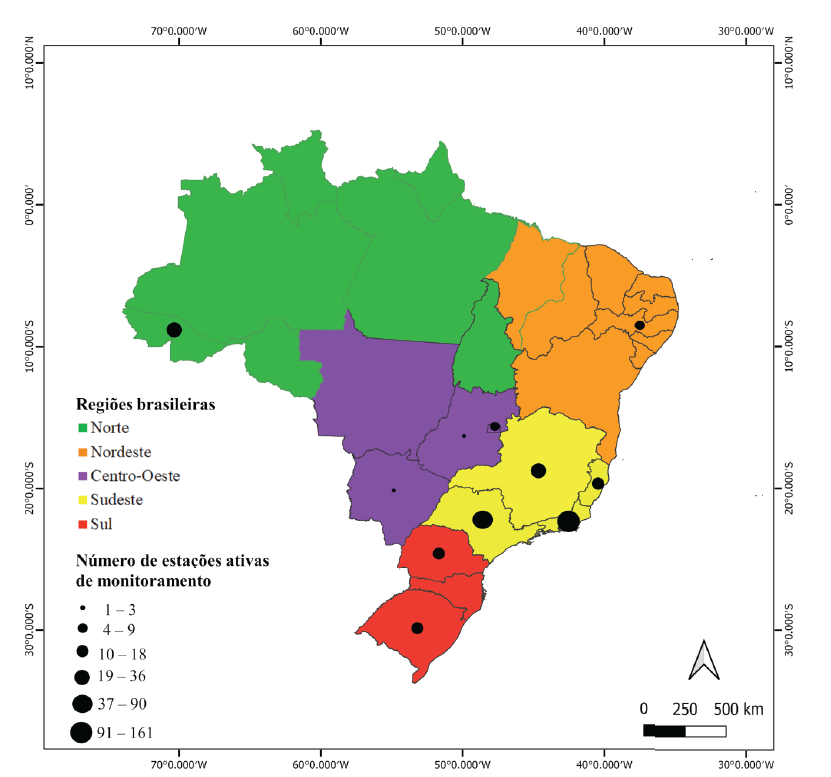
\includegraphics[width=\textwidth]{chapters/1-MONITORAMENTO/Figuras/Monitoramento BR Vormittag.png}
        \caption{Número de estações ativas no Brasil em 2021}
        \label{fig:monit-stations-br-2021}
        \fonte{\cite{Vormittag2021AnaliseBrasil}}
    \end{subfigure}
    \hfill
    \begin{subfigure}{0.5\textwidth}
        \includegraphics[width=\textwidth]{chapters/1-MONITORAMENTO/Figuras/Estações de referencia Brasil.png}
        \caption{Número de estações ativas no Brasil em 2022}
        \label{fig:monit-stations-br-2022}
        \fonte{\cite{Ferreira2022}}
    \end{subfigure}
    \hfill
    \label{fig:monit-stations-br}
\end{figure}

A pesar da sua elevada confiabilidade, a distribuição espacial limitada das redes de monitoramento de referência as habilita para proverem apenas informações globais, relativas a níveis de concentração de fundo \cite{Kumar2015}. Isto dificulta a compilação de informação confiável e representativa de áreas específicas. Esse fato constitui uma limitante para o estudo dos processos associados à poluição atmosférica. Dada a alta variabilidade espaço-temporal da concentração dos poluentes, especialmente em ambientes urbanos \cite{Mead2013TheNetworks}, a resolução espacial das redes de monitoramento é tão relevante quanto a confiabilidade das suas estações \cite{Jiao2016CommunityStates}.

Diante disso, se faz necessário a busca de novas soluções que possibilitem incrementar o número de monitores viáveis nas redes de monitoramento sem afetar a qualidade das medições. Todavia, especial cuidado deve ser tomado para não comprometer a qualidade dos dados obtidos, já que, como apontado por Emily Snyder e colaboradores, ter dados pouco confiáveis é mais prejudicial do que não ter dados, pois podem conduzir a decisões desacertadas \cite{Snyder2013}.